% 2008 年四川卷文科第 19 题：平面 ABEF ⊥ 平面 ABCD，两个直角梯形 ABEF、ABCD，
%   ∠BAD = ∠FAB = 90°，BC ∥= ½AD，BE ∥= ½AF，G、H 为 FA、FD 中点。
% 来源 PDF：gaokaomath-src/普通高考/2008/2008四川文.pdf
% SHA-256：1ba08ce1f61bedd8f036654d1054bebc1fda2ff655e05813ee4a45c552cc9c3e
% 原页：2008四川文.pdf 第 2 页（A3 三栏）第 1 栏，书页码 486。
% 绘图方式：按直角坐标建系后作斜投影 (x,y,z) -> (x+0.8y, 0.5y+z)，再整体缩放。
%   取 A(0,0,0)、B(2,0,0)、C(2,2,0)、D(0,4,0)、F(0,0,4)、E(2,0,2)，
%   则 G(0,0,2)、H(0,2,2)；底面 ABCD 的 AD、AC 与体对角线 AE、GH 用虚线。
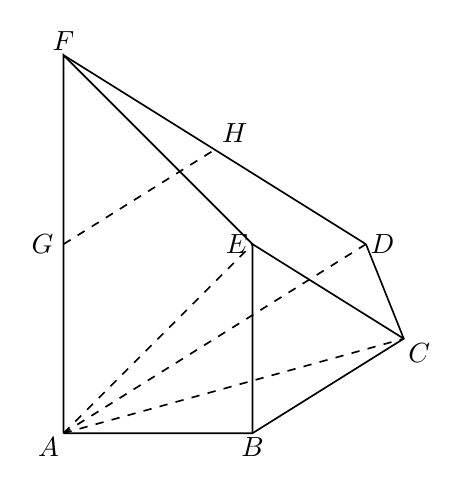
\begin{tikzpicture}[scale=1.2, semithick, every node/.style={inner sep=1.4pt}]
  \coordinate (A) at (0.00,0.00);
  \coordinate (B) at (2.00,0.00);
  \coordinate (C) at (3.60,1.00);
  \coordinate (D) at (3.20,2.00);
  \coordinate (F) at (0.00,4.00);
  \coordinate (E) at (2.00,2.00);
  \coordinate (G) at (0.00,2.00);
  \coordinate (H) at (1.60,3.00);

  % 底面 ABCD
  \draw (A) -- (B) -- (C) -- (D);
  \draw[dashed] (D) -- (A);
  \draw[dashed] (A) -- (C);

  % 立面 ABEF
  \draw (A) -- (F) -- (E) -- (B);

  % 侧棱与内部虚线
  \draw (C) -- (E);
  \draw (D) -- (F);
  \draw[dashed] (A) -- (E);
  \draw[dashed] (G) -- (H);

  \node[below left] at (A) {$A$};
  \node[below] at (B) {$B$};
  \node[below right] at (C) {$C$};
  \node[right] at (D) {$D$};
  \node[above] at (F) {$F$};
  \node[left] at (E) {$E$};
  \node[left=2pt] at (G) {$G$};
  \node[above right=1pt] at (H) {$H$};
\end{tikzpicture}
